\documentclass{article}
\usepackage[margin=0.2in,paperwidth=9in,paperheight=5.2in]{geometry}
\pagestyle{empty}
\usepackage{amsmath,amssymb}
\usepackage{tikz}
\usetikzlibrary{shapes.geometric, arrows.meta, positioning, calc}

\begin{document}
\noindent
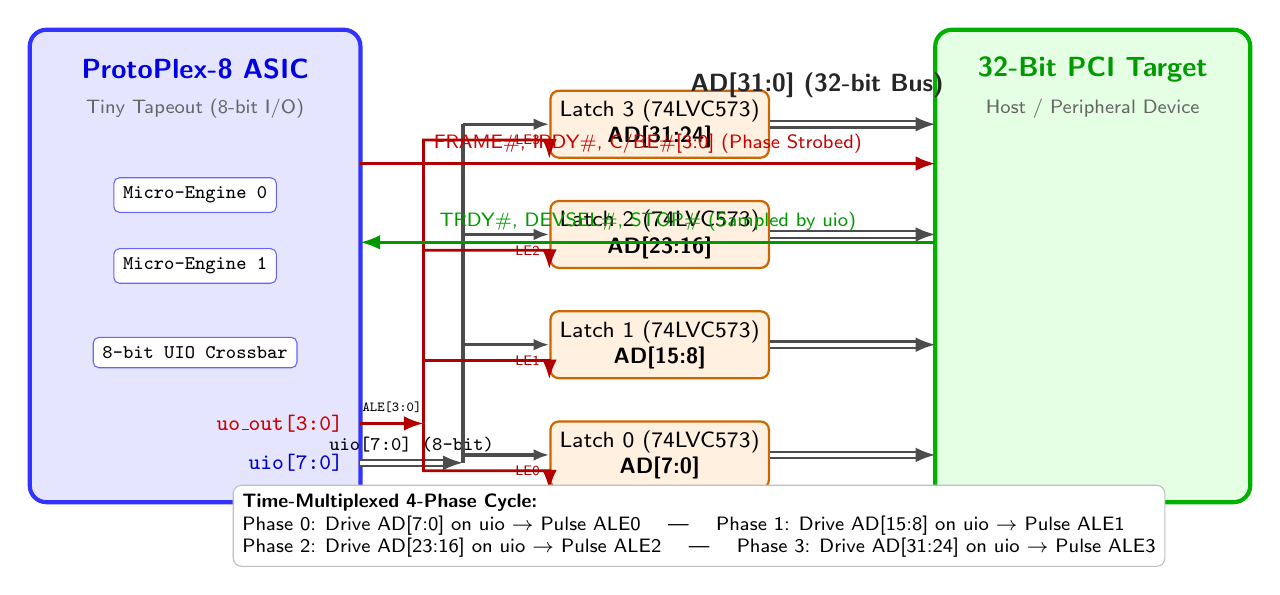
\begin{tikzpicture}[
    box/.style={draw=black!80, fill=blue!8, thick, rounded corners=3pt, minimum width=2.4cm, minimum height=1.0cm, align=center, font=\small\sffamily},
    latch/.style={draw=orange!80!black, fill=orange!12, thick, rounded corners=3pt, minimum width=2.2cm, minimum height=0.8cm, align=center, font=\footnotesize\sffamily},
    bus/.style={draw=black!70, double, double distance=1.5pt, line width=0.8pt, -{Latex[length=2.5mm]}},
    sig/.style={draw=red!70!black, line width=1pt, -{Latex[length=2.5mm]}},
    txt/.style={font=\scriptsize\sffamily}
]

% ProtoPlex-8 ASIC
\draw[fill=blue!10, draw=blue!80, line width=1.5pt, rounded corners=6pt] (0, 0.5) rectangle (4.2, 6.5);
\node[font=\bfseries\sffamily, text=blue!90!black] at (2.1, 6.0) {ProtoPlex-8 ASIC};
\node[font=\scriptsize\sffamily, text=gray!80!black] at (2.1, 5.5) {Tiny Tapeout (8-bit I/O)};

% Internal Blocks
\node[draw=blue!60, fill=white, rounded corners=2pt, font=\scriptsize\ttfamily] at (2.1, 4.4) {Micro-Engine 0};
\node[draw=blue!60, fill=white, rounded corners=2pt, font=\scriptsize\ttfamily] at (2.1, 3.5) {Micro-Engine 1};
\node[draw=blue!60, fill=white, rounded corners=2pt, font=\scriptsize\ttfamily] at (2.1, 2.4) {8-bit UIO Crossbar};

% Demux Strobe Outputs
\node[font=\footnotesize\ttfamily, red!80!black, anchor=east] at (4.1, 1.5) {uo\_out[3:0]};
\node[font=\footnotesize\ttfamily, blue!80!black, anchor=east] at (4.1, 1.0) {uio[7:0]};

% 4 Octal Latches (74LVC573)
\foreach \i/\lbl/\ad in {
    3/{Latch 3 (74LVC573)}/{AD[31:24]},
    2/{Latch 2 (74LVC573)}/{AD[23:16]},
    1/{Latch 1 (74LVC573)}/{AD[15:8]},
    0/{Latch 0 (74LVC573)}/{AD[7:0]}
} {
    \node[latch] (l\i) at (8.0, 1.1 + \i*1.4) {\lbl \\ \textbf{\ad}};
}

% Multiplexed 8-bit bus fanout
\draw[bus] (4.2, 1.0) -- (5.5, 1.0) node[midway, above, font=\scriptsize\ttfamily] {uio[7:0] (8-bit)};
\draw[line width=1.5pt, black!70] (5.5, 1.0) -- (5.5, 5.3);
\foreach \i in {0,1,2,3} {
    \draw[-{Latex[length=2mm]}, line width=1.2pt, black!70] (5.5, 1.1 + \i*1.4) -- (l\i.west);
}

% Latch strobe lines ALE0..ALE3
\draw[sig] (4.2, 1.5) -- (5.0, 1.5) node[midway, above, font=\tiny\ttfamily] {ALE[3:0]};
\foreach \i in {0,1,2,3} {
    \draw[sig] (5.0, 1.5) |- (6.6, 0.9 + \i*1.4) -- (l\i.south west);
    \node[font=\tiny\sffamily, red!70!black, anchor=east] at (6.6, 0.9 + \i*1.4) {LE\i};
}

% 32-bit PCI Target Device
\draw[fill=green!10, draw=green!70!black, line width=1.5pt, rounded corners=6pt] (11.5, 0.5) rectangle (15.5, 6.5);
\node[font=\bfseries\sffamily, text=green!60!black] at (13.5, 6.0) {32-Bit PCI Target};
\node[font=\scriptsize\sffamily, text=gray!80!black] at (13.5, 5.5) {Host / Peripheral Device};

% Latch to Target 32-bit Bus
\foreach \i in {0,1,2,3} {
    \draw[bus] (l\i.east) -- (11.5, 1.1 + \i*1.4);
}
\node[font=\small\bfseries\sffamily, text=black!85] at (10.0, 5.8) {AD[31:0] (32-bit Bus)};

% Control Handshake Lines
\draw[sig] (4.2, 4.8) -- (11.5, 4.8) node[midway, above, font=\scriptsize\sffamily, red!80!black] {FRAME\#, IRDY\#, C/BE\#[3:0] (Phase Strobed)};
\draw[{Latex[length=2.5mm]}-, draw=green!60!black, line width=1pt] (4.2, 3.8) -- (11.5, 3.8) node[midway, above, font=\scriptsize\sffamily, green!60!black] {TRDY\#, DEVSEL\#, STOP\# (Sampled by uio)};

% Protocol Phases Box
\node[draw=gray!50, fill=white, rounded corners=3pt, font=\scriptsize\sffamily, align=left] at (8.5, 0.2) {
    \textbf{Time-Multiplexed 4-Phase Cycle:} \\
    Phase 0: Drive AD[7:0] on uio $\rightarrow$ Pulse ALE0 \quad | \quad Phase 1: Drive AD[15:8] on uio $\rightarrow$ Pulse ALE1 \\
    Phase 2: Drive AD[23:16] on uio $\rightarrow$ Pulse ALE2 \quad | \quad Phase 3: Drive AD[31:24] on uio $\rightarrow$ Pulse ALE3
};

\end{tikzpicture}
\end{document}
